\documentclass[12pt]{extarticle}
\usepackage{geometry}
\geometry{a4paper, margin=1in}
\usepackage[utf8x]{inputenc}
\usepackage{graphicx}
\usepackage{listings}
\usepackage{authblk}
\usepackage{amsmath}
\usepackage{amsfonts}
\usepackage{enumitem}
\usepackage{caption}
\usepackage{amssymb}
\usepackage{hyperref}
\usepackage{setspace} % for line spacing adjustment

\lstnewenvironment{bashcode}[1][]{
    \lstset{
        language=bash,
        frame=single,
        frameround=tttt,
        framesep=5pt,
        framerule=0.8pt,
        basicstyle=\small,
        % rulecolor=\color{black},
        #1
    }
    \setstretch{0.95}
}{}

\title{\textbf{Mini Projet} 

Structures de Données\\
LU2IN006 }
\author{Maëlle LIU 21204734 - Thibaut MARCQ 21202966}
\date{21 Février 2024}

\begin{document}
\maketitle
\renewcommand*\contentsname{Sommaire}
\tableofcontents

\newpage
\section*{Explication de notre projet}
\addcontentsline{toc}{section}{Explication de notre projet}
\subsection*{Nature du projet}
\addcontentsline{toc}{subsection}{Nature du projet}
Le sujet de ce mini-projet visait à \textbf{modéliser une bibliothèque}. Une première partie était consacrée à la modélisation par une \textbf{liste chaînée}, une seconde partie était consacrée à la modélisation par une \textbf{table de hachage}. 
\\ \\
Dans chaque partie des fonctionnalitées étaient demandées : \textbf{charger un nombre de livres} dans la bibliothèque à partir d'un fichier, \textbf{afficher} la bibliothèque, \textbf{ajouter}/\textbf{supprimer} un livre dans la bibliothèque, \textbf{rechercher} un livre par : son \textbf{numéro}, son \textbf{titre} ou son \textbf{auteur}, \textbf{fusionner} deux bibliothèques dans une seule, rechercher les livres en \textbf{plusieurs exemplaires} et \textbf{enregistrer} la bibliothèque dans un fichier.
\subsection*{Organisation du projet}
\addcontentsline{toc}{subsection}{Organisation du projet}
Notre projet est structuré dans un seul dossier, dans le répertoire Projet3-4. Dans ce répertoire se trouve pour chaque partie, des fichiers .c et .h :
\begin{itemize}[label=-]
    \item les fichiers de la première partie sont identifiables par leur \textbf{suffixe \texttt{LC}},
    \item ceux de la deuxième partie sont identifiables par leur \textbf{suffixe \texttt{H}},
    \item ceux de la troisième partie ont un \textbf{préfixe \texttt{ex3}}.
\end{itemize}
Tous les fichiers sont compilables facilement grâce au Makefile. Celui-ci génère les fichiers .o ainsi que les exécutables \texttt{main}, \texttt{ex3-1} et \texttt{ex3-3}.
\\ \\
Le fichier \texttt{main} contient les main des deux premières parties, chacun distinguable lors du lancement du programme (option 1 ou 2). Les fichiers de l'exercice 3 correspondent à la question qui leur est associée.

\newpage
\section*{Réponses aux questions de l'exercice 3}
\addcontentsline{toc}{section}{Réponses aux questions de l'exercice 3}
\subsection*{Question 1}
\addcontentsline{toc}{subsection}{Question 1}
Voici les résultats que l'on obtient à la suite des mesures sur nos fonctions :
\begin{bashcode}
Liste Chainee, Recherche par num (cas livre present): 0.000098s
Table Hachage, Recherche par num (cas livre present): 0.000193s
Liste Chainee, Recherche par num (cas livre absent): 0.000114s
Table Hachage, Recherche par num (cas livre absent): 0.000313s

Liste Chainee, Recherche par titre (cas livre present): 0.000176s
Table Hachage, Recherche par titre (cas livre present): 0.000203s
Liste Chainee, Recherche par titre (cas livre absent): 0.000163s
Table Hachage, Recherche par titre (cas livre absent): 0.000367s

Liste Chainee, Recherche par auteur (cas livre present): 0.000197s
Table Hachage, Recherche par auteur (cas livre present): 0.000002s
Liste Chainee, Recherche par auteur (cas livre absent): 0.000198s
Table Hachage, Recherche par auteur (cas livre absent): 0.000001s
\end{bashcode} 
{\small Résultats obtenus sur une bibliothèque de taille \textbf{5000}} \\ \\
D'après ces résultats, on peut voir que la \textbf{liste chainée est la plus performante} pour les recherches par \textbf{numéro} et par \textbf{titre} : dans les deux cas considérés elle est plus rapide (recherche num présent: \texttt{0.000095s}, recherche num absent: \texttt{0.000199s}, recherche titre présent: \texttt{0.000027s}, recherche titre absent: \texttt{0.000204s}). \\ \\
En revanche, pour la recherche par \textbf{auteur}, la \textbf{table de hachage est la plus performante} (recherche auteur présent: \texttt{0.000195s}, recherche auteur absent : \texttt{0.000197s}). La recherche se fait presque instantannément avec elle.
\subsection*{Question 2}
\addcontentsline{toc}{subsection}{Question 2}
Voici les résultats obtenus en augmentant la taille de la bibliothèque :
\begin{bashcode}
Liste Chainee, Recherche par num (cas livre present): 0.001247s
Table Hachage, Recherche par num (cas livre present): 0.003058s
Liste Chainee, Recherche par num (cas livre absent): 0.001046s
Table Hachage, Recherche par num (cas livre absent): 0.004173s

Liste Chainee, Recherche par titre (cas livre present): 0.001490s
Table Hachage, Recherche par titre (cas livre present): 0.001632s
Liste Chainee, Recherche par titre (cas livre absent): 0.001132s
Table Hachage, Recherche par titre (cas livre absent): 0.003309s

Liste Chainee, Recherche par auteur (cas livre present): 0.001350s
Table Hachage, Recherche par auteur (cas livre present): 0.000008s
Liste Chainee, Recherche par auteur (cas livre absent): 0.001228s
Table Hachage, Recherche par auteur (cas livre absent): 0.000008s
\end{bashcode} 
{\small Résultats obtenus sur une bibliothèque de taille \textbf{40000}} \\ \\
Ces résultats confirment nos premières observations et les accentuent. La liste chainée est toujours \textbf{plus performante} sur la \textbf{recherche par numéro et par titre} mais ne l'est \textbf{pas lors de la recherche par auteur}. \\ \\
En comparaison avec les premiers résultats obtenus sur une bibliothèque plus petite, le temps de calcul de la recherche par auteur n'a \textbf{pas augmenté dans les mêmes proportions} que celui des autres recherches (avec ou sans table de hachage). Il est resté \textbf{très faible}. Ceci est dû à la \textbf{clé} de notre Table de Hachage. Celle-ci est basée sur l'\textbf{auteur} des livres de notre bibliothèque. Ainsi, cela rend les opérations sur les auteurs très rapides.
\\
\subsection*{Questions 3 et 4}
\addcontentsline{toc}{subsection}{Questions 3-4}
Détermination du temps de recherche des \textbf{ouvrages en plusieurs exemplaires}\\ \\
{\small (Q. 3)}\\
En redirigeant le code de \texttt{ex3-3.c} dans un fichier texte, on peut obtenir (dans GnuPlot) le graphique suivant: 

\begin{center}
\begin{figure}[h] % "h" spécifie que l'image doit être placée ici si possible
  \centering % Centre l'image
  \fbox{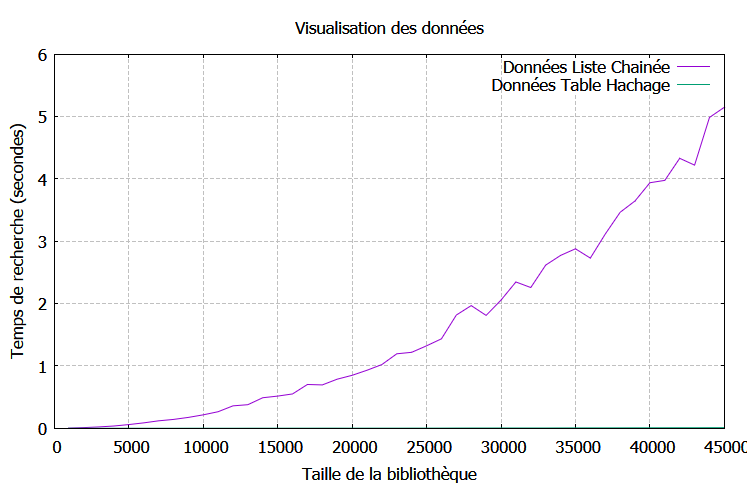
\includegraphics[width=0.75\linewidth]{pas1000-big.png}} % Insère l'image dans un cadre
  \captionsetup{justification=centering} % Centrer la légende
  \caption{Evolution des \textbf{temps de recherche} des deux structures \\ en fonction de la \textbf{taille de la bibliothèque} (pas de 1000)} % Ajoute une légende à l'image
  \label{fig:exemple} % Ajoute une étiquette pour faire référence à l'image
\end{figure}
\end{center}
D'après ce graphique, on peut voir que \textbf{plus la taille de la bibliothèque augmente}, plus le \textbf{temps de recherche} pour la fonction en Liste Chainée\textbf{ augmente} aussi. On ne distingue que \textbf{très peu} l'évolution des données de la Table de Hachage.\newpage
Pour mieux visualiser l'évolution des \textbf{recherches par Table de Hachage} :
\begin{center}
\begin{figure}[h] % "h" spécifie que l'image doit être placée ici si possible
  \centering % Centre l'image
  \fbox{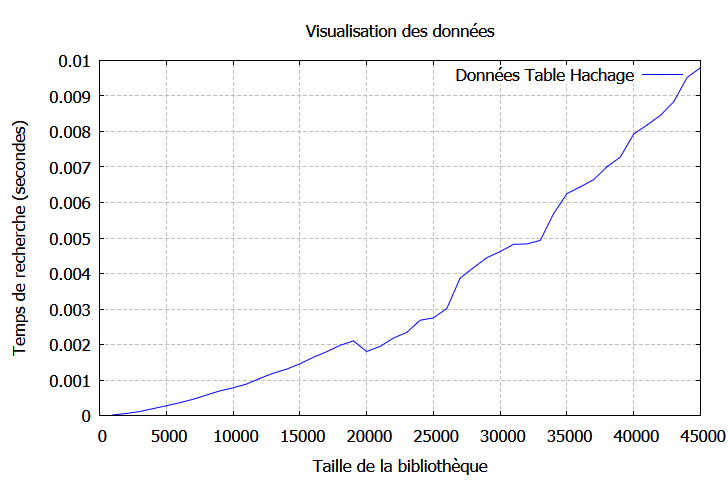
\includegraphics[width=0.75\linewidth]{graph-recherchePls-hachage.png}} % Insère l'image dans un cadre
  \captionsetup{justification=centering} % Centrer la légende
  \caption{Evolution des \textbf{temps de recherche} de la \textbf{Table de Hachage} \\ en fonction de la \textbf{taille de la bibliothèque} (pas de 1000)} % Ajoute une légende à l'image
  \label{fig:exemple} % Ajoute une étiquette pour faire référence à l'image
\end{figure}
\end{center} 
Ce graphique permet de visualiser \textbf{plus précisément} l'évolution des temps de recherche des livres en plusieurs exemplaires par la table de hachage. On se rend compte d'une \textbf{augmentation très faible} du temps de recherche. Contrairement à celle sur la Liste Chainée, qui évoluait sur \textbf{[0, 6] secondes}, celle sur la Table de Hachage évolue seulement sur \textbf{[0, 0.1] secondes}.\\ \\
{\small (Q. 4)}\\
Ceci est dû à la \textbf{complexité des deux fonctions} de recherche utilisées ici. La fonction en Liste Chainée a une \textbf{complexité temps pire-cas en $O(n^2)$}, tandis que celle en Table de Hachage a une complexité temps pire-cas \textbf{plus faible}. Pour chercher les livres en plusieurs exemplaires, elle s'intéresse en premier aux \textbf{livres qui ont le même auteur}. Comme nous l'avons vu à la question précédente, la \textbf{recherche par auteur} dans une Table de Hachage est très performante.



\end{document}


% cc